% !TeX root = Report.tex
\documentclass[12pt]{article}

% Package imports (organized and deduplicated)
\usepackage{biblatex}
\usepackage{changepage}
\usepackage{color}
\usepackage{enumitem}
\usepackage{float}
\usepackage{graphicx}
\usepackage{listings}
\usepackage{sectsty}
\usepackage{xcolor}
\usepackage[breaklinks=true]{hyperref}
\usepackage{xurl}
\usepackage{tikz}
\usepackage{lipsum}
\usepackage[format=plain,
            labelfont=it,
            textfont=]{caption}
\usetikzlibrary{shapes.geometric, arrows, positioning, calc}
\usepackage{./timing-diagrams}
\usetikzlibrary{calc}
\setcounter{biburlnumpenalty}{100}
\setcounter{biburlucpenalty}{100}
\setcounter{biburllcpenalty}{100}

\newcommand{\subsubsubsection}[1]{\paragraph{#1}\mbox{}\\}
\setcounter{secnumdepth}{4}
\setcounter{tocdepth}{4}

\newcommand{\writersnote}[1]{\marginpar{\small{\textcolor{blue}{Writer's note:}} \scriptsize\textit{#1}}}

% \usepackage{background}
% \backgroundsetup{
%   position=current page.north west,
%   angle=0,
%   nodeanchor=north west,
%   vshift=-1cm,
%   hshift=1cm,
%   color=red,
%   opacity=1,
%   scale=1,
%   contents={Preprint}
% }

\definecolor{darkblue}{RGB}{0, 0, 102} 
\hypersetup{
    colorlinks=true,
    pdfborder={0 0 0},
    linkbordercolor=white,
    urlcolor=darkblue,
    linkcolor=darkblue,
    citecolor=darkblue,
    filecolor=darkblue
}

% Make bibliography ragged right instead of justified
\AtBeginDocument{
  \renewcommand{\bibsetup}{\raggedright}
}
% Document configuration
\restylefloat{table}
\graphicspath{{./images/}}
\addbibresource{Library.bib}
\subsectionfont{\fontsize{12}{14}\selectfont}

% Author information
\author{
    Group Number: 107\\
    Joar Heimonen, Christian Vu, Naly Keli \\
    \texttt{contact@joar.me}\\ 
    \texttt{chvu002@student.kristiania.no}\\
    \texttt{nake002@student.kristiania.no}
}

% Title configuration
\title{
  \textbf{Preliminary Title}\\
  \large{Preliminary Description}
}
\date{\today}

\newcommand{\license}{
    \vspace{1em}
    \noindent\small{© 2025 Joar Heimonen,  Christian Vu, Naly Keli\\
    This work is licensed under a \href{https://creativecommons.org/licenses/by-sa/4.0/}{Creative Commons Attribution-Sharealike 4.0 International License}.}
}
\begin{document}
\maketitle

\begin{abstract}
  Preliminary Abstract
\end{abstract}

\pagebreak

\tableofcontents

\pagebreak


\section{Introduction}
There are many paradigms of commercial sensor management and monitoring. Organizations use among other things
PLC (programmable Logic Controllers), IoT devices and SCADA (Supervisory Control and Data Acquisition) systems to 
manage and monitor their sensors. For commercial use 
some of these alternatives are more popular than others. There are also a large amount of different higher level protocols
like MQTT, HTTP and SNMP that can be used to manage and monitor sensors. We propose using the NETCONF protocol 
with YANG sensor models for management. This work will be done in collaboration with Lightside Instruments AS.
\\
\\
This document will cover the following three topics:
\begin{itemize}
  \item \textbf{Work Methodology:} An indept analysis of the knowledge base around work methods like Scrum, Kanban, and Waterfall. 
  With a focus on how our work methodology differs from these.
  \item \textbf{NETCONF and YANG sensor management}: A qualitative analysis of the NETCONF and YANG protocols and how they can be used to manage sensors and 
  a description of our work with Lightside Instruments AS on NETCONF and YANG sensor management.
  \item \textbf{NETCONF Security}: A qualitative analysis of the security aspects of the NETCONF protocol.
\end{itemize}

\section{Lightside Instruments AS}
Lightside Instruments is a company specializing in developing instruments with model based network management 
for use in networking, network interconnect testing and telemetry. 
They design their instruments with YANG (RFC7950) \cite{bjorklundYANG11Data2016} models and NETCONF (RFC6241) \cite{ennsNetworkConfigurationProtocol2011} protocol. 
The instruments are based on IETF standards and drafts, 
and are implemented with software tools available in Debian, programmable 
logic and open hardware \cite{LightsideInstrumentsYANG}.

\section{Technical background}

\subsection{NETCONF and YANG}
NETCONF \cite{ennsNetworkConfigurationProtocol2011} is a model based Network Configuration Protocol.
Each NETCONF device presents the aquiring device with a YANG \cite{bjorklundYANG11Data2016} data model
consisting of the device state and parameters. 
Each data model has a set of constraints making them error correcting.

\subsection{Yuma123}
Yuma123 \cite{vassilevVlvassilevYuma1232025} is an open source NETCONF and YANG implementation.
Yuma123 is available as a Debian package and is maintained by Lightside Instruments AS.

\subsection{NodeJS}
Node.js \cite{NodejsRunJavaScript} is a JavaScript runtime built on Chrome's V8 JavaScript engine.
It is used to build JavaScript applications that can run independently of a web browser.
Node.js is popular for building server-side applications as it is relatively performant and 
it allows developers to work with the same language on both the client and server.

\subsection{Node-Yuma123}
Node-Yuma123 \cite{Nodeyuma1232025} is a NodeJS package that implements a set of Yuma123 bindings.
It allows for efficient NETCONF and YANG development in NodeJS.

\subsection{Node-RED}
Node-RED \cite{LowcodeProgrammingEventdriven} is an open source low code programming tool for event driven applications.
It is developed by IBM and is based on Node.js \cite{NodejsRunJavaScript}.
Node-RED is used to connect hardware devices and APIs through a visual programming interface.

\subsection{Grafana}
Grafana \cite{GrafanaOpenComposable} is an open source data visualization tool.
It is used to visualize arbitrary data from different data sources.

\subsection{XML and XPATH}
XML stands for Extensible Markup Language \cite{ExtensibleMarkupLanguage}. It is a
markup language that is used to encode data in a format that is both human and machine readable.
XPATH \cite{XMLPathLanguage} is a language for navigating XML documents.
An XPATH expression allows for the selection of arbitrary nodes in an XML document.

\subsection{Scrum}
Scrum \cite{HomeScrumorg} is a framework for agile \cite{AgileSoftwareDevelopment2025} software development. 
The term Scrum is derived from the game of rugby, where a scrum is a way of restarting play after a minor infringement \cite{ScrumRugbyUnion2025}.

\subsection{Kanban}
Kanban \cite{Kanban2025} is a framework for agile software development.
The term Kanban is derived from the Japanese word for "signboard" or "billboard" \cite{KanbanDevelopment2025}.

\subsection{Waterfall}
Waterfall \cite{WaterfallModel2025} is a framework for software development.
The waterfall model is a linear and sequential approach to software development.

\subsection{Extreme Programming}
Extreme Programming \cite{ExtremeProgramming2025} is a framework for agile software development.
Extreme Programming takes the best practices of software development and takes them to the extreme, hence the name.

\section{Work Methodology}

\subsection{Research Question}
This review examines the claims that Scrum, Kanban, Waterfall, Extreme Programming and DevOps 
increases worker productivity substantiated by empirical evidence.

\subsection{Scoping Review}

\subsubsection{Search strategy}
The following is our search strategy for the scoping review.
We will be searching for quantitative studies on the efficiency of the following work methodologies:
\begin{itemize}
  \item Scrum
  \item Kanban
  \item Waterfall
  \item Extreme Programming
  \item DevOps
\end{itemize}
We will be searching the following databases:
\begin{itemize}
  \item IEEE Xplore \cite{IEEEXplore}
  \item ACM Digital Library \cite{ACMDigitalLibrary}
  \item Google Scholar \cite{GoogleScholar} (Meta database)
\end{itemize}
We will also be searching the following industry websites:
\begin{itemize}
  \item Agile Alliance \cite{AgileAlliance2015}
  \item Scrum.org \cite{HomeScrumorg}
  \item DevOps Institute \cite{Organisations}
  \item Scrum Alliance \cite{ScrumAllianceFind}
\end{itemize}
Our search will consists of a set of primary and secondary keywords.
The primary keywords are:
\begin{itemize}
  \item Scrum
  \item Kanban
  \item Waterfall
  \item Extreme Programming
  \item DevOps
\end{itemize}
The secondary keywords are:
\begin{itemize}
  \item Effectiveness
  \item Efficiency
  \item Productivity
  \item Performance
  \item Success
  \item Failure
\end{itemize}
The search will be done using the following search string:

\begin{adjustwidth}{-4em}{0pt}
\begin{verbatim}
       (Scrum OR Kanban OR Waterfall OR "Extreme Programming" OR DevOps) 
                                      AND
(Effectiveness OR Efficiency OR Productivity OR Performance OR Success OR Failure)
\end{verbatim}
\end{adjustwidth}

\subsubsection{Exclusion Criteria}
The systematic review will include articles meeting the following criteria:
\begin{itemize}
  \item Published after January 1, 2020
  \item Published in English
  \item Relevant to the research question
  \item Empirical evidence
  \item Quantitative studies
  \item One of the 20 first results from each database
  \item Evaluating the effectiveness of the following methodologies:
  \begin{itemize}
    \item Scrum
    \item Kanban
    \item Waterfall
    \item Extreme Programming
    \item DevOps
  \end{itemize}
\end{itemize}

\subsubsection{Result}
After applying the exclusion criteria to a set of 60 articles, we discovered that 4 of them were duplicates.
The 56 remaining articles were screened by title and abstract, resulting in 12 articles being excluded.
The 44 remaining articles were assessed for eligibility, resulting in 33 articles being excluded.
The 11 remaining articles were included in the review.

\subsubsubsection{PRISMA flow diagram}
\textit{Figure \ref{fig:prisma}} shows the PRISMA \cite{PRISMAStatement} flow diagram for the scoping review.
The PRISMA flow diagram is a standardized way of reporting the results of a scoping review.

\begin{figure}
  \centering
  \begin{adjustwidth}{-4em}{0pt}
  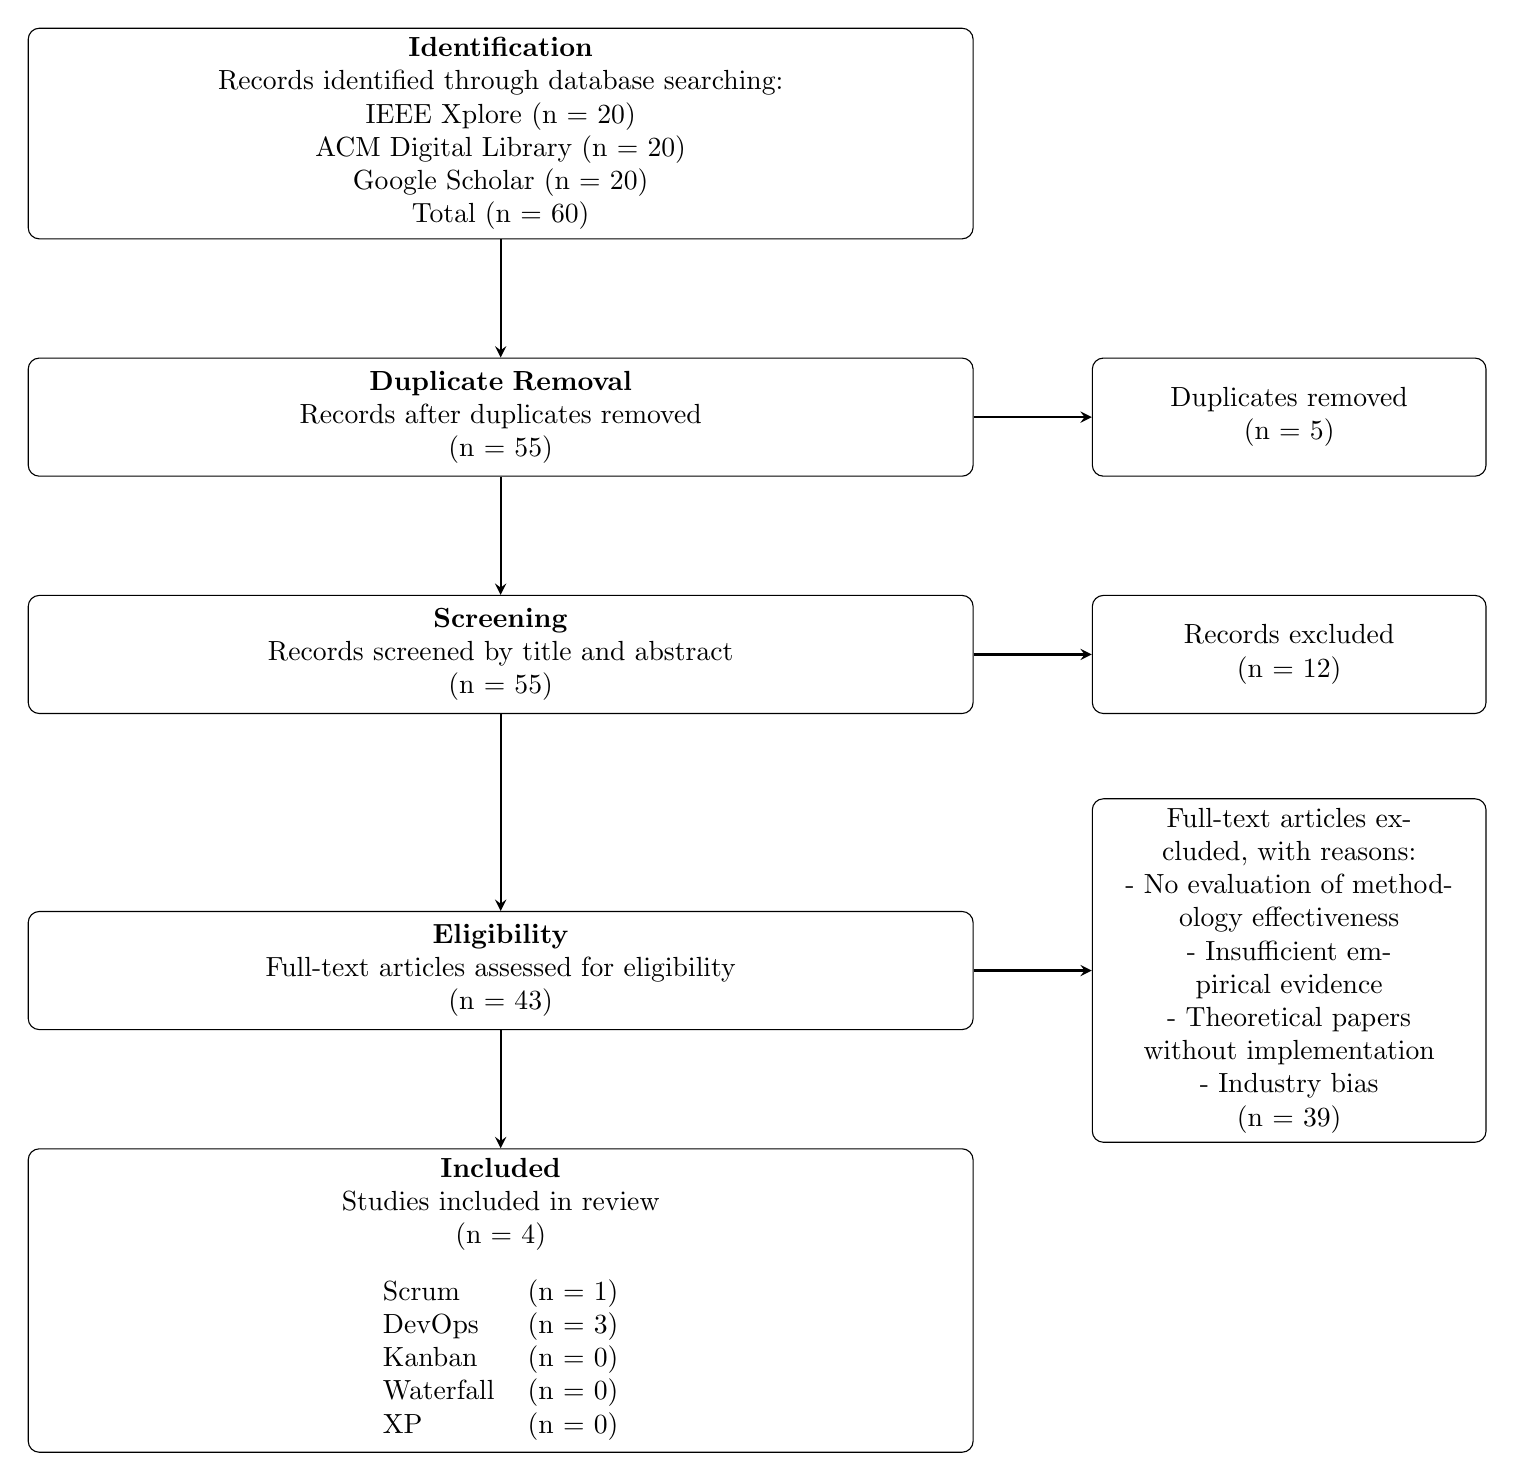
\begin{tikzpicture}[
   node distance = 1.5cm,
   box/.style = {draw, rectangle, rounded corners, minimum width=12cm, minimum height=1.5cm, text width=11.5cm, align=center},
   sidebox/.style = {draw, rectangle, rounded corners, minimum width=5cm, minimum height=1.5cm, text width=4.5cm, align=center},
   line/.style = {draw, -stealth, thick}
   ]
  % Identification box
  \node[box] (identification)
   {\textbf{Identification} \\
   Records identified through database searching:\\
   IEEE Xplore (n = 20)\\
   ACM Digital Library (n = 20)\\
   Google Scholar (n = 20)\\
   Total (n = 60)};
  
  % Duplicates removal box
  \node[box, below=of identification] (duplicates)
   {\textbf{Duplicate Removal} \\
   Records after duplicates removed\\
   (n = 55)};
  \node[sidebox, right=1.5cm of duplicates] (excluded0)
   {Duplicates removed\\
   (n = 5)};
  
  % Screening boxes
  \node[box, below=of duplicates] (screening)
   {\textbf{Screening} \\
   Records screened by title and abstract\\
   (n = 55)};
  \node[sidebox, right=1.5cm of screening] (excluded1)
   {Records excluded\\
   (n = 12)};
  
  % Eligibility boxes
  \node[box, below=2.5cm of screening] (eligibility)
   {\textbf{Eligibility} \\
   Full-text articles assessed for eligibility\\
   (n = 43)};
  \node[sidebox, right=1.5cm of eligibility] (excluded2)
   {Full-text articles excluded, with reasons:\\
   - No evaluation of methodology effectiveness\\
   - Insufficient empirical evidence\\
   - Theoretical papers without implementation\\
   - Industry bias\\
   (n = 39)};
  
  % Included box
  \node[box, below=of eligibility] (included)
   {\textbf{Included} \\
   Studies included in review\\
   (n = 4)\\[0.3cm]
  \begin{tabular}{ll}
   Scrum & (n = 1)\\
   DevOps & (n = 3)\\
   Kanban & (n = 0)\\
   Waterfall & (n = 0)\\
   XP & (n = 0)
  \end{tabular}};
  
  % Arrows
  \draw[line] (identification) -- (duplicates);
  \draw[line] (duplicates) -- (screening);
  \draw[line] (screening) -- (eligibility);
  \draw[line] (eligibility) -- (included);
  \draw[line] (duplicates) -- (excluded0);
  \draw[line] (screening) -- (excluded1);
  \draw[line] (eligibility) -- (excluded2);
  \end{tikzpicture}
  \end{adjustwidth}
  \caption{PRISMA flow diagram for scoping review of software development methodologies}
  \label{fig:prisma}
\end{figure}
  

\newpage

\subsection{Scrum}
Scrum is a framework for agile software development. The term Scrum is derived 
from the game of rugby, where a scrum is a way of restarting play after a minor infringement \cite{ScrumRugbyUnion2025}.
The use of the term Scrum in software development was first introduced by Takeuchi and Nonaka in 1986 in a paper titled 
"The New New Product Development Game" \cite{NewNewProduct}.
In the paper, the authors argue for a new approach to product development where the different stages of development are 
overlapped, rather than sequentially executed in a "pass the baton" fashion. This differs from 
the then popular NASA type PPP (Phased Project Planning) model \cite{PhasedProjectPlanning1968}.
\\
\\
Modern Scrum development consists of a set of sprints, these sprints consists of a pre-defined set of tasks
that are to be completed in the pre-defined sprint time frame. Each task or "story" is assigned an arbitrary number of points
that represents the complexity of the task. The sprint is the completed when there a no more points to be completed or the time frame is up.
There are many modern flavors of Scrum, like Accenture's \cite{AccentureLetThere} Autoscrum
which is a scrum framework that was first introduced in the talk "AGILE TRANSFORMATION?
FOR COMPLEX SYSTEMS?
...NO WAY!" by Brehm \cite{brehmAGILETRANSFORMATIONCOMPLEX2025} as can be seen in \textit{Figure \ref{fig:autoscrum}}.
Or the scaled agile framework (SAFe) \cite{Framework} which is a framework developed by Scaled Agile Incorporated  which introduces 
SAFe Scrum see \textit{Figure \ref{fig:sAFE}}.
Or the Deloitte's \cite{DeloitteAuditConsulting} "The Agile Landscape v3" that consists 
of all the different frameworks and methods used for project management. See the Scrum section in \textit{Figure \ref{fig:the_agile_landscape}}.

\begin{figure}
  \centering
  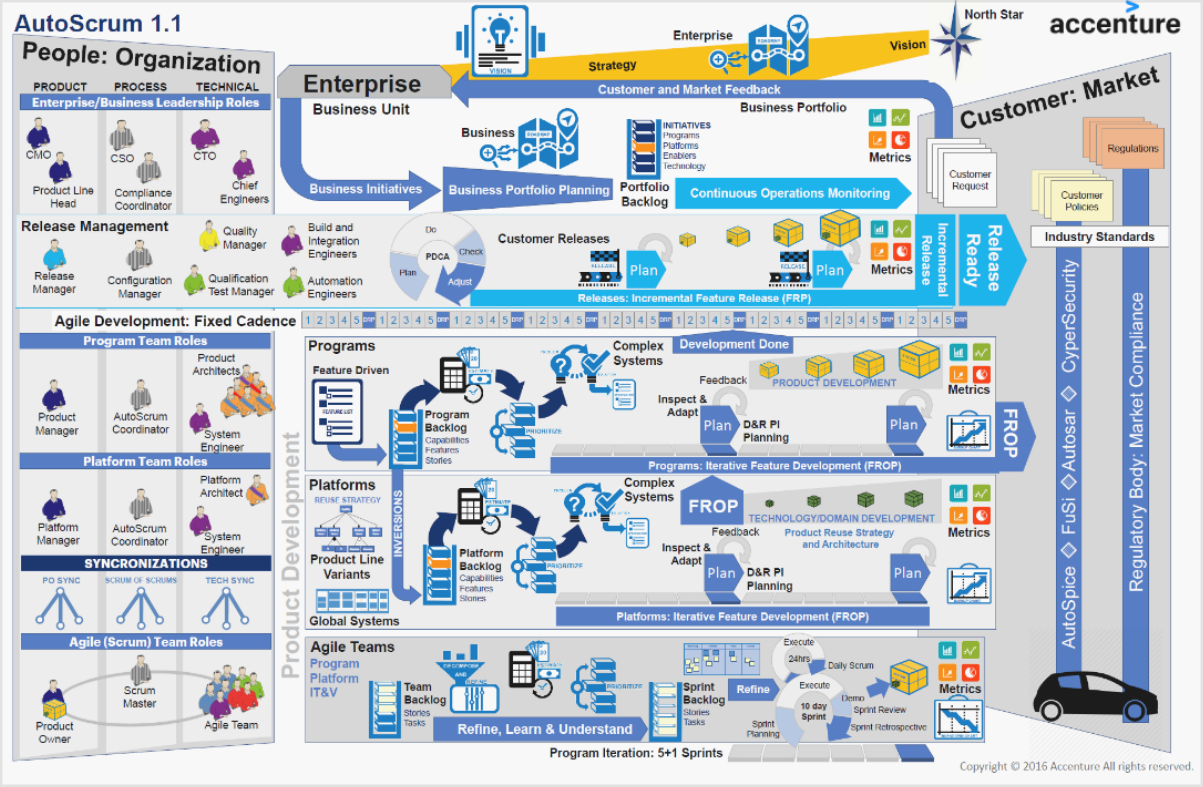
\includegraphics[width=\textwidth]{autoscrum.png}
  \caption{Excerpt from the presentation "AGILE TRANSFORMATION? FOR COMPLEX SYSTEMS? ...NO WAY!" by Brehm \cite{brehmAGILETRANSFORMATIONCOMPLEX2025} showing the Autoscrum framework.}
  \label{fig:autoscrum}
\end{figure}

\begin{figure}
  \centering
  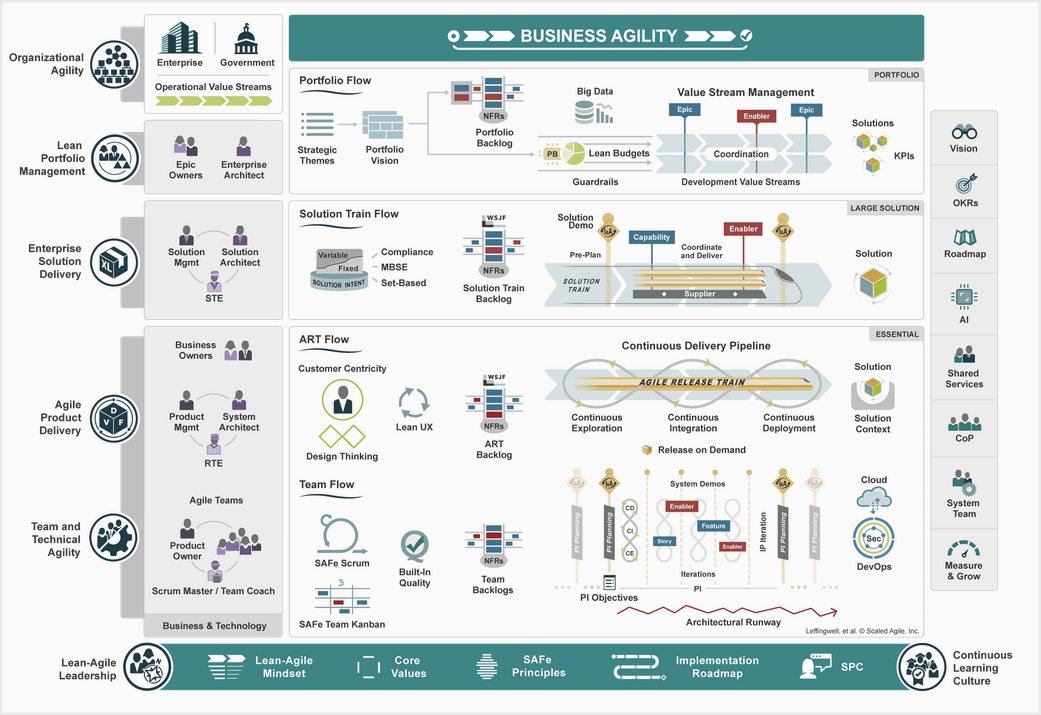
\includegraphics[width=\textwidth]{sAFE.png}
  \caption{The Scaled Agile Framework (SAFe) \cite{Framework}.}
  \label{fig:sAFE}
\end{figure}

\begin{figure}
  \centering
  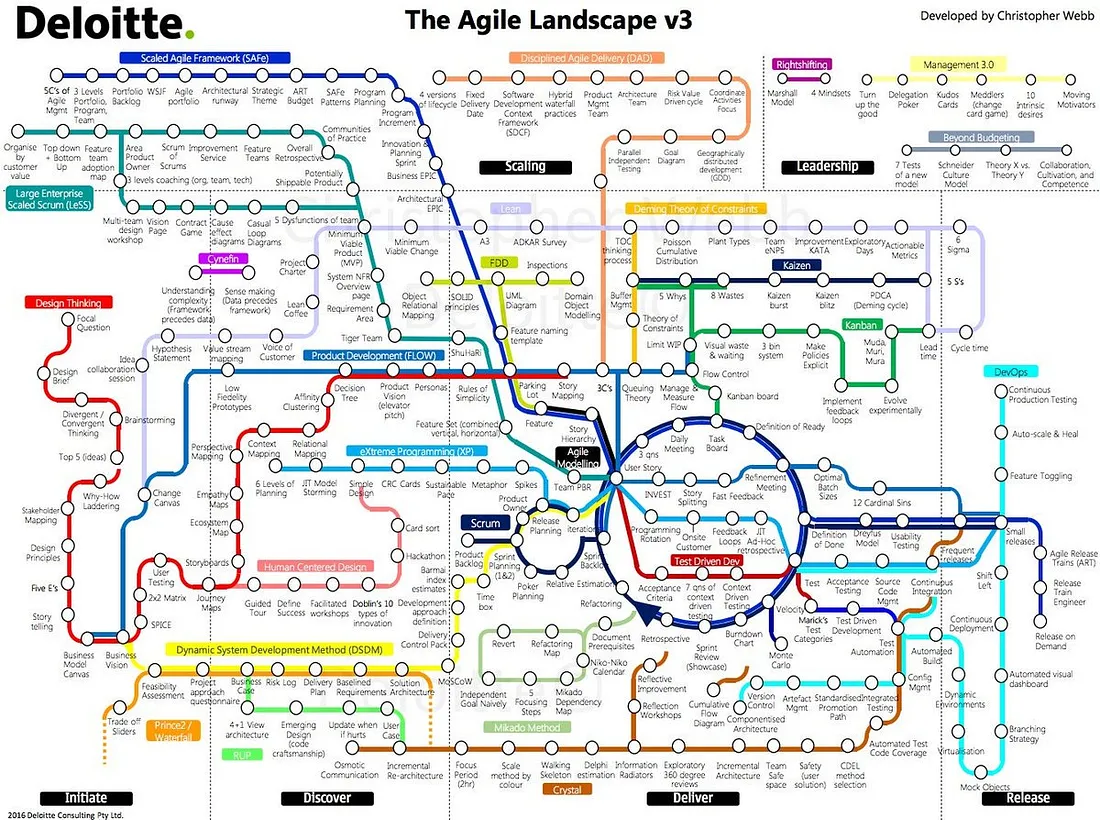
\includegraphics[width=\textwidth]{the_agile_landscape.png}
  \caption{The Agile Landscape v3 \cite{DeloitteAuditConsulting} showing the different frameworks and methods used for project management.}
  \label{fig:the_agile_landscape}
\end{figure}

\newpage

\subsubsection{Evidentiary foundation}
With only one article "A Theory of Scrum Team Effectiveness" by Verwijs and Russo \cite{verwijsTheoryScrumTeam2023} we can conclude that there
is no empirical evidence that Scrum increases worker productivity or efficiency. Whilst the findings of the article seems promising, and the article is thorough, there simply is not 
enough research on the topic to comment on the evidentiary foundation of Scrum, this is something taken in too account by the authors of the article. 
Only a handful of other articles have been published on the topic, but most of them fall outside the exclusion criteria of the scoping review as they
have been published before 2020.

\subsection{Kanban}
Kanban is a framework for agile software development. The term Kanban is derived from the Japanese word for "signboard" or "billboard" \cite{KanbanDevelopment2025}.
A Kanban board is a visual representation of the tasks that need to be completed, the board consists of multiple columns that represent the 
different stages of the development process. As a task is worked on it traverses the columns of the board until it is completed.
This provides a visual representation of the state of the project and allows for easy identification of bottlenecks in the process.
Kanban is a much more flexible and lean approach to project management than Scrum, as it follows closer to the agile manifesto's principles 
of flexibility and adaptability \cite{ManifestoAgileSoftware}.

\subsubsection{Evidentiary foundation}
With no articles found in the scoping review we can conclude that there is no empirical evidence that Kanban increases worker productivity or efficiency.

\subsection{Waterfall}
The waterfall \cite{WaterfallModel2025} is a linear and sequential approach to software development. Sets of tasks are grouped into phases, 
where each phase must be completed before the next phase can begin. This is reminiscent of the NASA type PPP 
(Phased Project Planning) model \cite{PhasedProjectPlanning1968}.
The waterfall model mirrors the traditional problem solving process, of breaking a problem down into a set of smaller problems,
and solving each of the smaller problems in a sequential manner. This is something that is found at the core 
of all project management methodologies.

\subsubsection{Evidentiary foundation}
With no articles found in the scoping review we can conclude that there is no empirical evidence that Waterfall increases worker productivity or efficiency.

\subsection{Extreme Programming}
Extreme Programming \cite{ExtremeProgramming2025} is a framework for agile software development. Extreme Programming takes 
the best practices of software development and takes them to the extreme, hence the name. A core part of Extreme Programming is the use of
pair programming \cite{PairProgramming2024}, where two developers work together on the same code.

\subsubsection{Evidentiary foundation}
With no articles found in the scoping review we can conclude that there is no empirical evidence that Extreme Programming increases worker productivity or efficiency.

\subsection{DevOps}
DevOps is the combination of development and operations, it is the practice of combining software development and IT operations.
This keeps the developers close to the day to day operations of the software they are developing. A result of developer operations is 
the use of automated continues integration and continues deployment (CI/CD) \cite{ContinuousDelivery2025} systems as the responsibility 
of the deployment falls on the developers. This methodology fosters early error detection and correction.

\subsubsection{Evidentiary foundation}
DevOps and Research Assessment (DORA) \cite{DORAGetBetter} is a research department at Google that focuses on 
researching assessment methods for DevOps. They publish a yearly report on the state of DevOps. Other than DORA independent research
into the topic is scarce and whilst research is being done there is currently not a strong enough evidentiary foundation to make 
any claims about the effectiveness of DevOps.

\subsection{Conclusion}
The scoping review has made it clear that there is a lack of research into the effectiveness of different work methodologies.
The industry seems focused on researching performance metrics for each methodology, rather than the 
effectiveness of the methodology itself.

\subsection{Our Work Methodology}
At Lightside Instruments we work with both hardware and software in a small team. 
This workflows lends a great deal of flexibility to our work.
With most engineers doubling as both hardware and software engineers, we have found it cumbersome to use a strict work methodology like most agile frameworks.
Due to the small size of our team we have adapted a DevOps like approach that is tailored for our needs. 
We have a set of tasks that are defined in a git repository. After a task is completed a pull request is submitted and the task
is marked as pending review. When the request is approved the task is marked as completed and the code is merged into the main branch.
We not only use automated continues integration and continues deployment (CI/CD) systems for our software, but also for our hardware.
We have developed a set of workflows that are used to automatically generate the production files for our hardware. 
\\
\\
Whilst there is no empirical evidence or any research suggesting that our work methodology is more effective than any of the other methodologies, 
we have found it to be a good fit for our needs. And we feel that it adheres close the principles set forth by the agile manifesto 
\cite{ManifestoAgileSoftware}.

\section{NETCONF and YANG sensor management}

Hardware management is an essential part of administrating a larger network. 
Together with Lightside Instruments AS we have 
developed open source tools for YANG and NETCONF aimed at hardware sensor management.
We have built a reference implementation of a NETCONF system that tackles this issue.
Our reference implementation consists two NETCONF temperature probes,
a data aggregator, a data visualization tool and
a tool for quick management of NETCONF devices.
\\
\\
The following sections will describe the project and how each of the components are implemented.
An illustration of the architecture of the project can be seen in \textit{Figure \ref{fig:architecture}}.

\begin{figure}
  \centering
  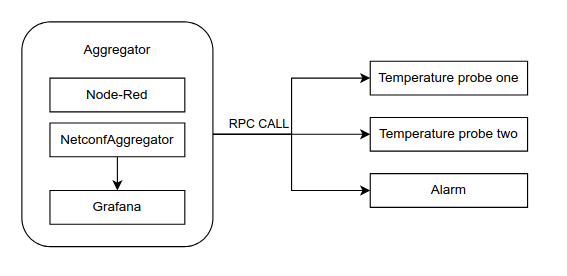
\includegraphics[width=\textwidth]{refimparch2.drawio.png}
  \caption{Architecture of the NETCONF and YANG sensor management system.}
  \label{fig:architecture}
\end{figure}

\newpage

\subsection{NETCONF}
NETCONF \cite{ennsNetworkConfigurationProtocol2011} is a mode based Network Configuration Protocol
implemented by the IETF (Internet Engineering Task Force) in the RFC (Request for Comments) 6241 \cite{ennsNetworkConfigurationProtocol2011}.

\subsection{YANG Model}
The YANG model is a model used to describe the state and actions of a NETCONF device.
The Internet Engineering Task Force (IETF) has developed a set of standard YANG models for NETCONF devices.
For the purposes of this project we will not be using the standard YANG models,
but instead we will be using a custom YANG model developed by Lightside Instruments AS that only 
describes the state of thermometers. See \textit{Figure \ref{fig:yang}} for the YANG model.
\begin{figure}
  \begin{verbatim}
    module lsi-thermometers {
      yang-version 1.1;
      namespace "urn:lsi:params:xml:ns:yang:thermometers";
      prefix thermometers;

      organization  "Lightside Instruments AS";

      description
        "Thermometers monitoring module.";

      revision 2022-07-25 {
        description
          "Initial version.";
      }

      container thermometers {
        config false;
        list thermometer {
          key "name";
          leaf name {
            type string;
          }
          leaf value {
            description
              "Temperature in degrees Celsius multiplied by 100.";
            type int32 {
              range "-27315..max";
            }
          }
        }
      }
    }
  \end{verbatim}
  \caption{YANG model for thermometer management}
  \label{fig:yang}
\end{figure}

\newpage

\subsection{Node-RED}
Node-RED is a low code programming tool for event driven applications.
It makes it possible to create arbitrary flows that function as a compatibility layer
between different systems and protocols. The low code nature of Node-RED makes arbitrary system
integration accessible even for the lay person.

\subsubsection{Red-Netconf}
Red-Netconf \cite{LightsideinstrumentsRednetconf} is a Node-RED plugin that implements the following two 
nodes:
\begin{itemize}
  \item \textbf{Netconf Session}: This node is used to create a NETCONF session with a NETCONF device.
  \item \textbf{Netconf Yangcli}: This node is used to send NETCONF commands to a NETCONF device using yangcli commands.
\end{itemize}
Using these two nodes we are able to create Node-RED flows that can manage NETCONF devices.

\subsubsubsection{Temperature alert}
As an example of how the Red-Netconf nodes can be used we created
a Node-RED reference flow that collects data from a thermometer and switches on an LED
when the temperature is above 25 degrees Celsius, this can be seen in \textit{Figure \ref{fig:red-netconf}}.

\newpage

\begin{figure}
  \centering
  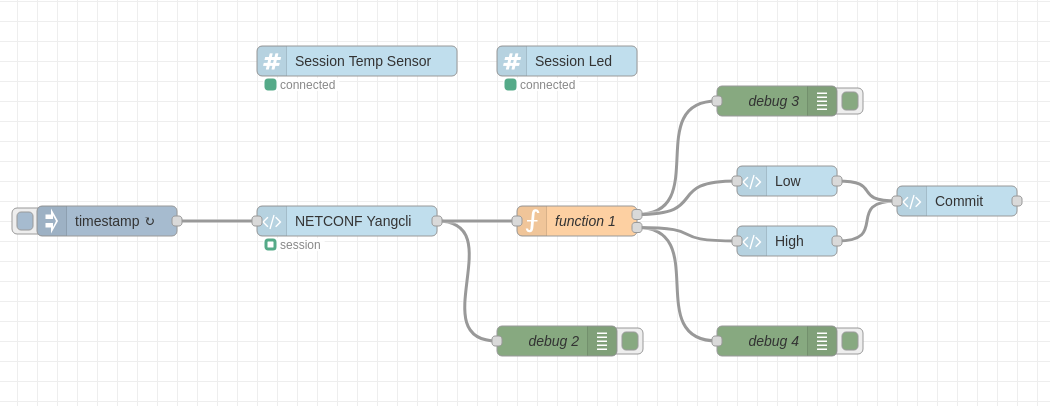
\includegraphics[width=\textwidth]{red-netconf.png}
  \caption{Node-RED flow using Red-Netconf nodes that monitors a temperature sensor and 
  switches on an LED when the temperature is above 25 degrees Celsius.}
  \label{fig:red-netconf}
\end{figure}


\subsubsection{Node-Yuma123}
Yuma123 is an implementation of the NETCONF standard that is written in C.
It consists of a NETCONF server written in C, an RPC (Remote Procedure Call) client 
and a YANGCLI interpreter. The YANGCLI interpreter is a command line tool that can be used to
interact with NETCONF devices using YANG models and YANGCLI commands. YANGCLI
translates the YANGCLI commands into NETCONF RPC calls and sends them to the NETCONF device.
Yuma123 also presents an API that can be used to interact with the NETCONF server called 
libyuma-dev.
\\
\\
Node-Yuma123 is a set of NodeJS bindings for the Yuma123 API. It is written in C++ and created
to resemble the original C API as closely as possible. Node-Yuma123 also implements some 
new functions like asynchronous connections. Implementing this was quite a challenge as the 
libyuma-dev API is not thread safe. Instead of running each connection in a new thread we
stack the instructions using libuv \cite{libuv} and run them in the main thread. This 
resolves most of our threading issues, but some issues still remain. 
These issues are related to how libyuma-dev allocates memory.


\subsubsubsection{easyNetconf}
C is a low level functional programming language, there are many implementations of the C compiler.
All of these implementations follow the C standard set forth by the American National Standards Institute 
(ANSI) in the ANSI C standard. Due to JavaScipts object-oriented nature we decided to create 
a wrapper around the node-Yuma123 library. This wrapper allows us to use the node-Yuma123
library in an object-oriented way.

\subsection{Grafana}
Grafana is an open source data visualization tool. Since its inception ins 2014 it has become the industry standard
for data visualization. It is used to visualize arbitrary data from different data sources.
We have developed a solution for fetching and visualizing arbitrary NETCONF data using Grafana.
We call this solution NetconfAggregator.

\subsubsection{NetconfAggregator}
NetconfAggregator is a NodeJS package that uses the easyNetconf wrapper 
\cite{heimonenSlenderman00Netconfaggregator2025} to aggregate NETCONF data and store 
it in a postgresql database. The data is stored in the form of a time series consisting of an ID, a timestamp and the 
raw XML data from the NETCONF device. This allows the data to be extracted and visualized using XPATH queries.
An example of this can be seen in \textit{Figure \ref{fig:netconf-aggregator-memfree}}.
This example shows how the query \textit{"//proc/meminfo/MemFree"} can be used to create a graph of the memory usage 
on a raspberry pi trough the NetconfAggregator datasource plugin in Grafana.
\\
\\
Figure \ref{fig:netconf-aggregator} shows the architecture of the NetconfAggregator, consisting
of a PostgreSQL database, a NetconfAggregator instance and a Grafana instance running the NetconfAggregator datasource plugin.
The NetconfAggregator gets the state of each NETCONF device using the YangCLI command \textit{"xget /"} which
fetches the state of the device. The response is then stored in the database.
When the NetconfAggregator receives a query from the datasource plugin it applies the specified XPATH to 
the relevant data-range in the database and returns the result to the datasource plugin.

\begin{figure}
  \centering
  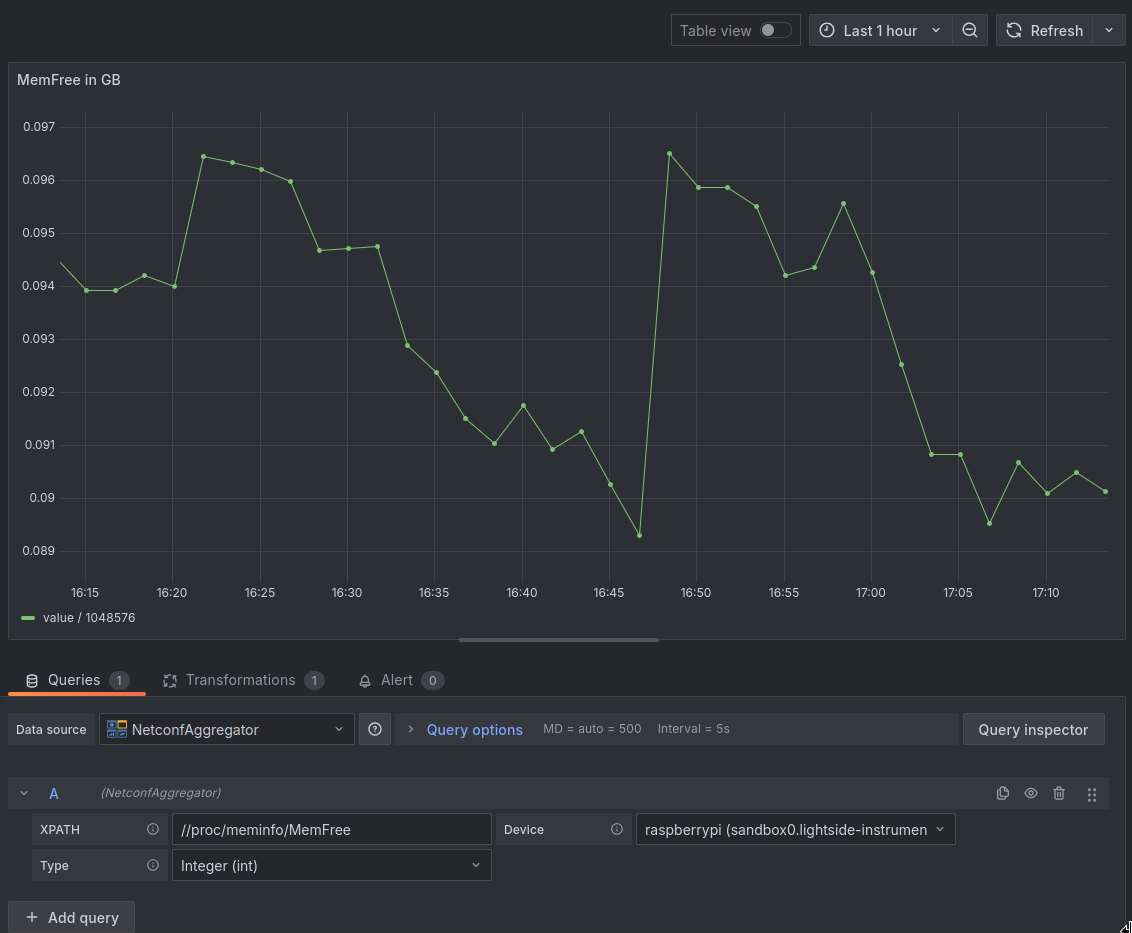
\includegraphics[width=\textwidth]{memfree.png}
  \caption{Querying the memory free data on a raspberry pi using XPATH and the NetconfAggregator plugin.}
  \label{fig:netconf-aggregator-memfree}
\end{figure}

\begin{figure}
  \centering
  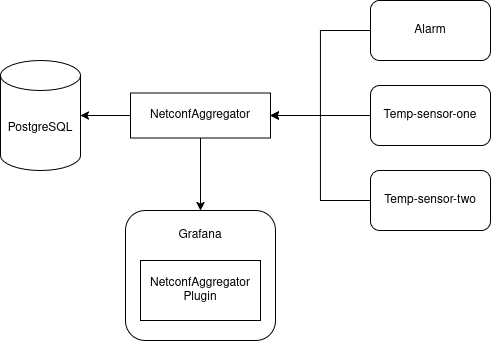
\includegraphics[width=\textwidth]{NetconfAggregator.png}
  \caption{NetconfAggregator architecture.}
  \label{fig:netconf-aggregator}
\end{figure}

\newpage

We quickly discovered that processing XPATHS is processor intensive. Especially when the data set is large.
Grafana also has a tendency to send all the queries belonging to a dashboard at once therefore, we decided 
to implement a caching system, where the results of the XPATH queries are cached in memory, stored in a hash table.
However, this did not work as expected, as the queries were arriving at the same time the responses did not 
have time to reach the cache before the next identical query arrived.
To solve this we implemented a queue system, we call it the event queue. 
When a query goes to processing it is simultaneously added to the event queue.
Future identical queries are delayed until the processing of the first query is completed.
A delay is added to each request that the server receives. This delay is based 
on the number of queries that are currently being processed, and thus makes
sure that no two identical queries are processed at the same time.
An illustration of how requests are processed can be seen in \textit{Figure \ref{fig:xpath-query}}.


\begin{figure}
  \centering
  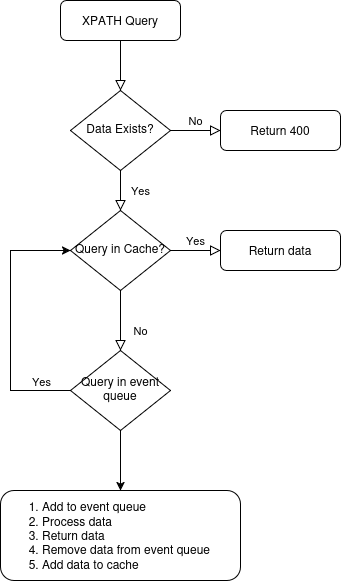
\includegraphics{xpathquery.drawio.png}
  \caption{XPATH query processing.}
  \label{fig:xpath-query}
\end{figure}


\newpage

\subsection{Decentralized monitoring}
We believe that the power of NETCONF lies in its ability to be used in a decentralized manner.
This means that multiple aggregators can be used to manage the same NETCONF devices. 
The example in \textit{Figure \ref{fig:decentralized-monitoring}} shows two servers each containing a node-red instance, a NetconfAggregator 
instance and a Grafana instance. The node-red instance and the NetconfAggregator functions completely independently of each other.
Thus making the monitoring system completely separate from the management system. The example consists of a normal networking setup
consisting of three NETCONF enabled switches, a NETCONF enabled temperature sensor and a NETCONF enabled alarm.
This architecture allows for arbitrary control and monitoring of the NETCONF devices using the NetconfAggregator and Node-RED.

\newpage

\begin{figure}
  \centering
  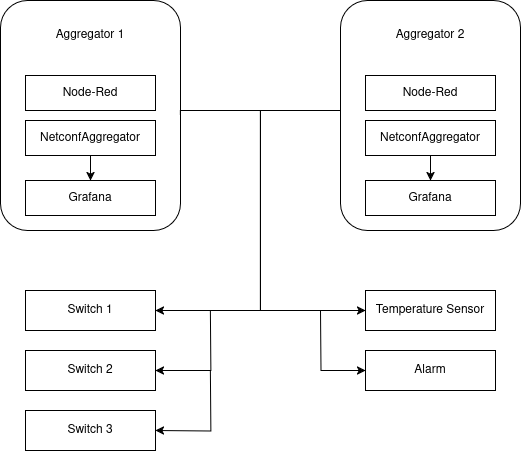
\includegraphics[width=\textwidth]{architecture1.png}
  \caption{Decentralized monitoring of NETCONF devices using Grafana, NetconfAggregator and Node-RED.}
  \label{fig:decentralized-monitoring}
\end{figure}

\newpage

\section{NETCONF Security}

\pagebreak
\addcontentsline{toc}{section}{References}
\printbibliography
\license
\end{document}
